\chapter{Energy balance with thermodynamic tabulations}
%\chaptermark{Energy Balance with thermodynamic tabulations}
\begin{nolinkcolors} 
\minitoc
\end{nolinkcolors}
\newpage
%
%
%=====================================
\section{State of the art}
%=====================================
To model macrosegregation during solidification, a minimum of four conservation equations are necessary:
conservation  of  mass, momentum,  chemical  species and  energy. The  phase  change
literature  contains a  wealth of numerical methods to solve energy conservation
in solidifying alloys. A comprehensive overview of these methods is given by \citet{swaminathan_enthalpy_1993}.

The corresponding equation associates the total average enthalpy to the
temperature  via  intrinsic  alloy  properties, such  as the heat  capacity of  the
phases and the latent  heat associated with the phase transformations. However, in the course
of solidification and while macrosegregation is taking place, these  properties change because the average
composition may  vary  significantly: the  transformation paths are thus modified, as well as
the phases' composition and heat capacity. Similarly, the latent heat of phase  transformations
is not a mere constant that could be distributed as a function of the phase fractions
assuming only temperature-dependent phases' properties, as often found in the literature \citep{bellet_call_2009}.
It is thus impossible to establish a priori the dependence of the enthalpy with respect
to temperature when macrosegregation alters the average composition, even in the case of full thermodynamic equilibrium
between phases. 

In this chapter, we discuss a suitable numerical scheme based on an enthalpy method,
already used in the literature  to  alleviate this macrosegregation-related problem \citep{swaminathan_enthalpy_1993,
carozzani_direct_2013}. Later on, we introduce a modified formulation, using the effective heat capacity method that 
increases the original scheme's efficiency. 

This chapter introduces an enthalpy method that makes use of a temperature-based solver. 
It uses tabulated thermodynamic quantities (solidification paths, phases' enthalpy  and composition) 
in a range of average compositions and temperatures as found in the literature 
\citep{dore_modelling_2000,thuinet_prediction_2004,du_modeling_2007}, 
with the aim of evaluating the total average enthalpy as well as the effective heat capacity. 
The novelty of the modified method resides in the use of thermodynamic tabulations without losing 
the advantages of the previous method, thus yielding faster computation times while maintaining a 
good accuracy.


%=====================================
\section{Thermodynamic considerations}
%=====================================

%-----------------------------
\subsection{Volume averaging} 
%-----------------------------

The volume averaging technique, presented in \cref{sec:volumeavg}, is considered
when solving the energy equation in the presence of macrosegregation. The reason is that phase
properties and distributions varying with the average composition, have a great impact on the average thermal properties,
and hence on the overall heat transfer in the system. We recall the basic equation:
%%-------------
\begin{align}
\label{eq:volume_average_psi}
& \avg{\psi} = \sum_\phi \gphi \avg{\psi}^{\phi}
\end{align}
%%-------------
where $g^\phi$ denotes the volume fraction of phase $\phi$ in the RVE. 
It should be emphasized that the averaging technique applies to virtually all thermodynamic volumetric variables (enthalpy, density $\dots$). 
Among these variables, the temperature is also considered to be uniform in the RVE. 

Applying the volume averaging technique to the energy 
conservation principle along with interfacial balances between the phases, results in the following averaged equation \citep{rappaz_numerical_2003}:
%%-------------
\begin{align}
\label{eq:averaged_energy_eqn}
& \frac{\d \rh}{\d t} + \nabla \cdot \rhv = \nabla \cdot \brac{\avg{\kappa} \nabvec T} + \avg{\dot{Q}_V}
\end{align}
%%-------------
where $\rho$ stands for the density, $h$ the mass enthalpy, $\vec{v}$ the velocity field, $\kappa$ the thermal conductivity, $T$ the temperature 
and $\dot{Q}_V$ a possible volumetric heat source. 
\Cref{eq:averaged_energy_eqn} is the standard averaged form of the energy conservation equation used in non-stationary phase 
change problems. 
%\comment{ I could elaborate more in this paragraph by showing the possible equations for the explicit formulation and maybe a figure to show the AlSi7
%computation that i did with a v small time step }
 
It is clear that the nature of the temperature-enthalpy relationship plays a central 
role when formulating the resolution strategy of this nonlinear equation. Generally, it is admitted that, depending on the resolution strategy, 
it is necessary to express enthalpy as a function of temperature or vice-versa, together with associated partial derivatives, 
$\frac{d \rh}{dT}$ or $\frac{dT }{d \rh}$.

It is noted that in the FEM context, the RVE is represented by a node in a finite element, so for instance the temperature in a RVE
is denoted $\Tj$ henceforth, where $j$ represents the index of the node localising the RVE.

%--------------------------------------------------------
\subsection{The temperature-enthalpy relationship} 
%--------------------------------------------------------

In solidification problems, additional variables are involved in \cref{eq:volume_average_psi} and \cref{eq:averaged_energy_eqn}, 
like the transformation path that defines the history of the phase fractions, as well as the average chemical composition $\wi$, 
i being the index of the chemical species (only the solutes are considered). The temperature-enthalpy relation averaged over the 
phases in a given RVE writes:
%%-------------
\begin{align}
\label{eq:volume_average_enthalpy}
& \rh = \sum_\phi \gphi_{\brac{T, \wi \dots}} \rphi_{\brac{T, \wi^{\phi} \dots}} \hphi_{\brac{T, \wi^{\phi} \dots}}
\end{align}
%%-------------

Note that the volume average enthalpy is approximated by the product $\avg{\rho h}^{\phi}=\hphi \rphi$ in the current work. As stated 
in the introduction, it becomes clear from \cref{eq:volume_average_enthalpy} that phase properties, i.e. average phase density, , $\rphi$ and enthalpy, $\hphi$, 
are temperature and composition dependent. This equation is the key to convert the average volume enthalpy to temperature (through a procedure named \emph{H2T}) 
or vice-versa (\emph{T2H}). The values of the different phase fractions $\gphi$ (solidification path) and phase enthalpies $\rh^{\phi}$ are thus needed 
to close the relation.

%--------------------------------------------------------
\subsection{Tabulation of properties}
%--------------------------------------------------------

The complexity of performing a thermodynamic conversion is directly linked 
to the simplicity of determining the alloy properties, namely the phase fractions 
and both phase densities and enthalpies. In the case of binary alloys and with several assumptions 
with respect to the system (e.g., linear monovariant lines in temperature-composition 
relationships of the phase diagram, constant heat capacity of phases and constant latent heat of transformations, 
equilibrium approximations between phases) analytical calculations are often used to determine 
the phase fractions and phase compositions. 
Nevertheless, analytical relations are more complex or even impossible to derive 
in the case of multicomponent alloys ($i>1$), or even for binary alloys with multiple phase transformations
(e.g. peritectic and eutectic reactions) with a nonlinear phase diagram. 

To overcome this problem, one can resort to 
thermodynamic databases and phase equilibrium calculations to tabulate the transformation paths 
and the phase densities and enthalpies for a given range of temperatures and average compositions. It is a handy 
solution for two main reasons: first, the conversion is merely a binary search in a table; secondly, 
it is a simple solution for coupling with macrosegregation. In this way, phase fractions $\gphi$ are 
tabulated as functions of temperature and average composition, while for each phase $\phi$ the mass 
enthalpy, $\hphi$, and the density, $\rphi$, are tabulated as functions of temperature and phase 
intrinsic average compositions $\wiphi$, as well as other possible parameters. 

\Cref{table:t2h_data} summarizes the 
steps in order to perform a temperature-to-enthalpy (\emph{T2H}) conversion using the predefined tabulation 
approach. 
In step 1, the transformation path is acquired for each average composition, $\wi$, and temperature, $T$, 
to determine the list of phases, their volume fractions $\gphi$ and their intrinsic compositions $\wi^{\phi}$, assuming
full equilibrium. In step 2, the phase enthalpy $\hphi$  and density $\rphi$ are determined by searching for the temperature and 
the already known phase composition $\wi^{\phi}$. In step 3, the average volume enthalpy is computed from the 
volume fraction, density and mass enthalpy of phases using \cref{eq:volume_average_enthalpy}. 
A flowchart explaining \emph{T2H} conversion steps is given in \cref{fig:algorithm_t2h}.

%---------------------------
% this table did not work when using custom tabulate env. because of the call to \cref ?
\begin{table}[htbp]
\centering
\caption{Tabulation processing for a \emph{T2H} procedure}
\label{table:t2h_data}
{\tabulinesep=1.0mm
\begin{tabu}{|c|c|c|c|}
\tabucline[1pt]{-}
\textbf{Step Number} 	& 	\textbf{1}		& \textbf{2}		& 	\textbf{3} 				\\\tabucline[1pt]{-}
\textbf{Inputs} 		&  ${T,\wi}$		& ${T,\wiphi}$		&	${\gphi, \rphi \hphi}$ \\
\textbf{Outputs} 		&  ${\gphi,\wiphi}$	& ${\rphi,\hphi}$	&	${\avg{\rho h}}$ (\cref{eq:volume_average_enthalpy})  \\\tabucline[1pt]{-}
\end{tabu}}
\end{table}
%---------------------------

The methodology to build the tabulations is straightforward. It is based on two main scans. On the one hand, intervals for the variation of the 
average composition $\wi$ are chosen from the known alloy composition. These variations have to cover the extreme values adopted during the 
simulation, which are not known a priori. An interval is also selected for the variation of temperature. The latter is easier to determine as it
usually starts from the initial melt temperature and goes down to the room temperature in a standard casting simulation. For each mapping of
composition and temperature, a thermodynamic equilibrium state is computed. The outputs are the 
number of phases encountered, together with their fraction and intrinsic compositions. 
On the other hand, for each phase, a scan of the intrinsic composition and temperature is made to compute the intrinsic 
properties. The same temperature interval and step as defined earlier are used.

Regarding the enthalpy-to-temperature conversion (\emph{H2T}) shown in the flowchart in \cref{fig:algorithm_h2t}, 
a backward iterative \emph{T2H} search is performed. 
For a known composition $\wi$, denoting $\brent$ the iteration index to convert the enthalpy 
$H_{\text{input}}$, we start with an initial guess for temperature $T^{\brentzero}$ then convert it to an 
enthalpy $H^{\brentzero}$ with the \emph{T2H} conversion. Using an appropriate nonlinear algorithm (Brent is the most versatile 
in our case), we aim at minimizing the following scalar residual: $R_{H} = \abval{H_{\text{input}} - H^\brent }$. 
Once the algorithm has converged, the temperature $T^\brent$ is the result of the \emph{H2T} conversion. It is 
inferred that the first conversion (\emph{T2H}) is a direct one whereas the latter (\emph{H2T}) is indirect and requires 
a series of iterative steps; each step being a single \emph{T2H} resolution. In other words, a \emph{H2T} conversion is a 
backward search for a temperature, hence it is slower. This conversion's speed lag is exacerbated when tabulations 
increase in size (e.g. large number of temperature and composition steps) and complexity (e.g., multicomponent 
industrial alloys used in casting), since the search gets more complicated with the increasing number of input 
columns (one column for each alloying element).

%-------------------------------------------------------------------------------------
\begin{figure}[htbp]
\newlength{\rightcol}
\setlength{\largeur}{9cm}
\setlength{\llargeur}{6cm}
\setlength{\rightcol}{5.5cm}
\centering
\begin{tikzpicture}[node distance=0.4cm]

\tikzstyle{rect}=[rectangle,draw,text=black]
\tikzstyle{whiterect}=[rectangle,text=black]
\tikzstyle{test}=[diamond,aspect=3,draw,text=black]
\tikzstyle{fleche}=[->,>=stealth]
\tikzstyle{trait}=[]
\setlength{\rlargeur}{\largeur}
\addtolength{\rlargeur}{-2.\tabcolsep}
\addtolength{\rlargeur}{-1.\llargeur}


\node[rect] (init) at (0cm,5cm)
{
	\begin{tabular}{@{}p{\llargeur}p{\rightcol}@{}}
		\textbf{Initialisation} \\
		Temperature 	& $\Tj$ \\
		Average composition & $\wi_j$ \\
	\end{tabular}
};

\node[rect,below=of init] (microseg)
{
	\begin{tabular}{@{}p{\llargeur}p{\rightcol}@{}}
		\textbf{Microsegregation law} \\		
		Phase fractions					& $(\Tj,\wi_j) \rightarrow g^\phi_j$ \\
		Phase compositions 				& $(\Tj,\wi_j) \rightarrow \wiphi_j$ \\
		Phase mass enthalpies			& $(\Tj,\wiphi_j) \rightarrow \hphi_j$ \\
		Phase densities 				& $(\Tj,\wiphi_j) \rightarrow \rphi_j$
	\end{tabular}
};
\draw[trait] (init) -- (microseg);

\node[rect,below=of microseg] (solve)
{
	\begin{tabular}{@{}p{\llargeur}p{\rightcol}@{}}
		\textbf{Total enthalpy} &	$ \rhoh_j=\sum_\phi \crochet{g^\phi_j \rphi_j \hphi_j}_{\Tj}$ \\
								&	(\cref{eq:volume_average_enthalpy})
	\end{tabular}
};
\draw[trait] (microseg) -- (solve);

\end{tikzpicture}
\caption{Algorithm for a single temperature to enthalpy (\emph{T2H}) conversion at node $j$.} \label{fig:algorithm_t2h}
\end{figure}
%-------------------------------------------------------------------------------------
%*************************************************************************************
%-------------------------------------------------------------------------------------
%*************************************************************************************
\begin{figure}[htbp]
\setlength{\largeur}{9cm}
\setlength{\llargeur}{6cm}
\setlength{\rightcol}{5.5cm}
\newcommand\Tjbrent{\ensuremath{T_j^\brent}}
\newcommand\Hjbrent{\ensuremath{\rhoh_j^\brent}}
\centering
\begin{tikzpicture}[node distance=0.5cm]

\tikzstyle{rect}=[rectangle,draw,text=black]
\tikzstyle{whiterect}=[rectangle,text=black]
\tikzstyle{test}=[diamond,aspect=3,draw,text=black]
\tikzstyle{fleche}=[->,>=stealth]
\tikzstyle{trait}=[]
\setlength{\rlargeur}{\largeur}
\addtolength{\rlargeur}{-2.\tabcolsep}
\addtolength{\rlargeur}{-1.\llargeur}


\node[rect] (init) at (0cm,5cm)
{
	\begin{tabular}{@{}p{\llargeur}p{\rightcol}@{}}
		\textbf{Initialisation} \\
		Enthalpy			& $\rhoh_j$ \\
		Old temperature 	& $\Tjtminus$ \\
		Average composition & $\wi_j$ \\
	\end{tabular}
};

\node[rect, below=of init] (brent_init)
{
	\begin{tabular}{@{}p{\llargeur}p{\rightcol}@{}}
		\textbf{Brent's initialisation} \\
		Iteration &	$\brentzero$ \\
		Temperature & $T^\brentzero = \Tjtminus$
	\end{tabular}
};
\draw[trait] (init) -- (brent_init);

\node[rect,below=of brent_init] (microseg)
{
	\begin{tabular}{@{}p{\llargeur}p{\rightcol}@{}}
		\textbf{Microsegregation law} \\		
		Phase fractions					& $(\Tjbrent,\wi_j) \rightarrow \crochet{g^\phi_j}^\brent$ \\
		Phase compositions 				& $(\Tjbrent,\wi_j) \rightarrow \crochet{\wiphi_j}^\brent$ \\
		Phase mass enthalpies 			& $(\Tjbrent,\wiphi_j) \rightarrow \crochet{\hphi}^\brent$ \\
		Phase densities 				& $(\Tjbrent,\wiphi_j) \rightarrow \crochet{\rphi}^\brent$ \\
	\end{tabular}
};
\draw[trait] (brent_init) -- (microseg);

\node[rect,below=of microseg] (TtoH)
{
	\begin{tabular}{@{}p{\llargeur}p{\rightcol}@{}}
		\textbf{\emph{T2H} conversion} & $\Tjbrent \rightarrow \Hjbrent $ \quad (\cref{fig:algorithm_t2h})
	\end{tabular}
};
\draw[trait] (microseg) -- (TtoH);

\node[rect,below=of TtoH] (residual)
{
	\begin{tabular}{@{}p{\llargeur}p{\rightcol}@{}}
		\textbf{Enthalpy residual} & $R_\text{Brent}^\brentplus = \abval{\rhoh_j - \Hjbrent }$
	\end{tabular}
};
\draw[trait] (TtoH) -- (residual);

\node[test,below=of residual] (test)
{
	$R_\text{Brent}^\brentplus < \varepsilon_\text{Brent}$
};
\draw[trait] (residual) -- (test);

\node[rect,below=of test] (update)
{
	\begin{tabular}{@{}p{\llargeur}p{\rightcol}@{}}
		\textbf{Conversion} & $T_j = \Tjbrent$
	\end{tabular}
};
\draw[trait] (test) -- (update);
%----
\coordinate[shift={(-3mm,0mm)}] (microsegwest) at (microseg.west);
\draw[fleche] (test.west) -| (microsegwest) -- (microseg);
\node[anchor=south east] (No) 	at (test.west) {No};
\node[anchor=north east] (iterate) at (test.west) {$\brent \leftarrow \brentplus$};

\end{tikzpicture}
\caption{Algorithm for a single enthalpy to temperature (\emph{H2T}) conversion at node $j$.} \label{fig:algorithm_h2t}
\end{figure}
%-------------------------------------------------------------------------------------
%*************************************************************************************
%-------------------------------------------------------------------------------------
%*************************************************************************************

%==================
\section{Numerical method}
%==================

% Once the variational form has been discretised in space and time, two possible resolution schemes emerge: the first is an 
% explicit forward Euler scheme which gives rise to a linear equation where the temperature is known at time $t$, $T^t$. This requires very small 
% time steps in the current context, which limits the solver's usability at the scale of industrial applications. The second scheme is the 
% backward Euler or full implicit discretisation where terms are function of $T^{t+\Delta t}$. It leads to a nonlinear equation with 2 interdependent 
% unknowns, $\rh^{t+\Delta t}$ and  $T^{t+\Delta t}$.

The finite element method is used to solve the energy conservation as expressed by \cref{eq:averaged_energy_eqn}. 
A test function $\test$ belonging to the Hilbertian Sobolev space $\hilbert(\OhmE)$ of continuous integrable test functions 
is used to formulate the integral variational form of \cref{eq:averaged_energy_eqn} \citep{suli_lecture_2000}. 
A Fourier boundary condition is considered on the domain boundary $\partial \OhmE$. The domain $\Ohm$
is discretised using first-order linear simplexes, $\OhmE$, defined by their number of local nodes, NbLoc: triangles 
in 2D with NbLoc=3 and tetrahedra in 3D with  NbLoc=4. The outcome is a residual that we aim to minimize so that the 
conservation principle is satisfied. Therefore, the weak form writes:
%----------------------
\begin{multline}
\label{eq:weak_energy}
\forall \test \in M=\curly{u \in \hilbert(\OhmE)} \\
\integral{\OhmE}{\test \tempup{H}}{V} 
 + \integral{\OhmE}{\test \vit \cdot \nabvec \avg{\rho h}^l}{V}
 - \integral{\OhmE}{\test \diff{\avg{\kappa}}{T} }{V}
 - \integral{\OhmE}{\test \source }{V}
 = 0
\end{multline}
%------------
where $H=\rho h$ is the volumetric enthalpy, introduced to simplify notations in the following. 
Furthermore, we assumed a static solid phase and an incompressible liquid phase, which allowed recasting the second term of 
\cref{eq:averaged_energy_eqn} into $\vit \cdot \nabvec \avg{\rho h}^l$. 
$\avg{\rho h}^l = \rhol \hl$ is not main variable of the energy conservation equation's weak form, \cref{eq:weak_energy}.
Therefore we express it as a function of temperature, which is related to the main variable
via the enthalpy-temperature relation: 
%----------------------
\begin{align}
\label{eq:enthalpy_advection}
\nabvec \avg{\rho h}^l = \nabvec \brac{\rhol \hl} = \rhol \cpl \nabvec T
\end{align}
%------------
where $\cpl$ is the mass heat capacity of the liquid phase. Ideally, this value should
be taken directly from the thermodynamic database if it is available. Otherwise, it can be derived by differentiation 
of the tabulated liquid mass enthalpy with respect to temperature. In this work, $\cpl$ is considered constant, 
equal to the alloy's initial mass heat capacity.  
The steps for discretising in time and space \cref{eq:weak_energy} are well detailed in  
some text books like \citet{rappaz_numerical_2003}. 
As for enthalpy and temperature, they are spatially discretised in each simplex 
using interpolations functions $\interp$, thus defining the nodal values $H_j$ and $T_j$, respectively: 
%----------------------
\begin{align}
\label{eq:discretise_H}
H 	&= \sum_{j=1}^{\text{NbLoc}}  \interp_j   \Hj \\ 
\label{eq:discretise_T}
T		&= \sum_{j=1}^{\text{NbLoc}}  \interp_j   \Tj
\end{align}
%------------
The Galerkin formulation gives the expression for the residual contribution at a mesh node $i$ (here $i$ is not the usual solute index)
for time step $t$ in a local element $\element$:
%----------------------
\begin{align}
\begin{split}
\label{eq:discretise_residual_local}
& \brac{R_i^E}^t = \Mij^E \brac{\Hjt - \Hjtminus} + \Aij^E \Tjt + \brac{\Kija^E + \Kijb^E}\Tjt -\Fi^E - \Qi^E=0 \\
& i,j:1 \rightarrow \text{NbLoc}
\end{split}
\end{align}
%------------
where the volumetric contributions are detailed as follows:
%----------------------
\begin{align}
& \textit{transient term:} \quad  \Mij^E = \integral{\OhmE}{\frac{1}{\dt} \interp_i \interp_j }{V} \\ 
& \textit{advection term:} \quad  \Aij^E = \integral{\OhmE}{\rhol \cpl \interp_i \vit \cdot \nabvec \interp_j}{V} \\ 
& \textit{diffusion term:} \quad  \Kija^E = \integral{\OhmE}{\avg{\kappa} \nabvec \interp_i\nabvec \interp_j}{V} \\ 
& \textit{source term:} \quad  \Qi^E = \integral{\OhmE}{\interp_i \source}{V}
\end{align}
%------------
while the surface boundary contributions are given by:
%-------
\begin{align}
& \textit{boundary condition term 1:}	\quad  \Kijb^E = \integral{\dOhmE}{\hext \interp_i \interp_j}{S} \\ 
& \textit{boundary condition term 2:}	\quad	\Fi^E = \integral{\dOhmE}{\hext \Text \interp_i}{S} \\
\end{align}
%-------
%
The surface integrals $\Kijb^E$ and $\Fi^E$ are related to a Fourier-type boundary condition, 
with $\hext$ as a coefficient of heat exchange and $\Text$ as the external temperature far from the 
boundary. The energy conservation principle is satisfied when the sum of the residual contributions 
coming from all the mesh elements is zero. In other words, the following global residual defined by 
the assembly of these contributions, should be minimized: 
%----------------------
\begin{align}
\begin{split}
\label{eq:discretise_residual_global}
& \brac{R_i}^t = \Mij \brac{\Hjt - \Hjtminus} + \Aij \Tjt + \brac{\Kija + \Kijb}\Tjt -\Fi - \Qi=0 \\
& i,j:1 \rightarrow \text{NbGlob}
\end{split}
\end{align}
%------------
where the global tensors $\Mij$, $\Aij$, $\Kija$ , $\Kijb$ , $\Fi$ and $\Qi$ contain respectively, after an assembly step, 
the contributions of the local matrices $\Mij^E$, $\Aij^E$, $\Kija^E$ , $\Kijb^E$ , $\Fi^E$ and $\Qi^E$ from each discretised 
element in the domain $\Ohm$. Accordingly, the indices $i$ and $j$ refer to global node numbers, where the total number of nodes is 
denoted by "NbGlob". 

It is clear that the global residual inherits the dependence between volumetric enthalpy and temperature. 
This is shown in \cref{eq:discretise_residual_global} where the average volume enthalpy is a function of the temperature. It infers that this residual 
is a non-linear function; therefore minimizing it requires an iterative non-linear algorithm. 

Our choice settles on the Newton-Raphson method, known for its quadratic convergence speed. A solidification problem can induce severe non-linearities 
from the release of the latent heat (which itself is temperature and composition dependent) and the variations of the average thermophysical 
properties of the alloy with respect to temperature, phase fraction and average composition. This algorithm could thus treat such variations. 
Considering the link between the properties and temperature, \cref{eq:discretise_residual_global} may be solved either for the average volumetric enthalpy 
or for the temperature as the nodal unknown, hence both formulations are presented hereafter.


%------------------------------------------------------
\subsection{Enthalpy-based approach }
%------------------------------------------------------

The residual is re-written using a Taylor series expansion to the first order for a nonlinear iteration $\iter$ :
%-----------------
\begin{align}
\label{eq:Hsolver_residual}
& \brac{R_i}^\iterplus = \brac{R_i}^\iter + \brac{\dRdH}^{\iter}_{ij} \Delta \Hj^\iter + \order\brac{\Hj^2}
\end{align}
%------------

Neglecting the second order terms, the suggested correction at each iteration in view of cancelling 
the residual and giving the new value $\Hj^\iter$, is given by the linear system in \cref{eq:Hsolver_residual_linear}
relative to what we call a \emph{Hsolver}:
%-----------------
\begin{align}
\label{eq:Hsolver_residual_linear}
& \brac{\dRdH}^{\iter}_{ij} \brac{\Hj^\iterplus - \Hj^\iter} = -R_i^\iter
\end{align}
%------------
where $\dRdH$ is a global tangent matrix yielding the variations of the residual with respect to the volumetric enthalpy 
in the previous iteration, $\Hj^\iter$. The detailed flow chart for the \emph{Hsolver} is given in \cref{fig:HsolverSteps}.
If \cref{eq:discretise_residual_local} is considered, then the contribution of an element $\OhmE$ writes:
%-----------------
\begin{align}
\label{eq:dRdH}
& \brac{\dRdH^E}^{\iter}_{ij} 
= \Mij^E 
+ \underbrace{\Aij^E \brac{\dTdH}^{\iter}_{j}}_{\nosum}
+ \underbrace{\brac{\Kija^E + \Kijb^E} \brac{\dTdH}^{\iter}_{j}}_{\nosum}
\end{align}
%------------
\Cref{eq:dRdH} is the core of the enthalpy-based solver. The resolution of \cref{eq:Hsolver_residual_linear} 
then yields a new estimate of the vector of nodal volumetric enthalpies $H^\iterplus$, which are the only unknowns to be solved for. 
Once determined at iteration $\iter$, convergence tests are performed.


%-----------------------------------------
\subsection{Temperature-based approach }
%-----------------------------------------

Similarly to the \emph{Hsolver}, the local residual is recast for a nonlinear iteration $\iter$, 
leading this time to an iterative temperature correction:
%-----------------
\begin{align}
\label{eq:Tsolver_residual_linear}
& \brac{\dRdT}^\iter_{ij} \brac{\Tj^\iterplus - \Tj^\iter} = -R_i^\iter
\end{align}
%------------
where $\dRdT$ is a global tangent matrix yielding the variations of the residual with respect to temperature $\Tj^\iter$ at the previous iteration. 
This solver will be referred to as \emph{Tsolver}. The corresponding flow chart is given in \cref{fig:TsolverSteps}.
The contribution of an element $\OhmE$ to this tangent matrix is evaluated as:
%-----------------
\begin{align}
\label{eq:dRdT}
& \brac{\dRdT^E}^{\iter}_{ij}
= \underbrace{\Mij^E \brac{\dHdT}^{\iter}_{j}}_{\nosum}
+ \Aij^E
+ \brac{\Kija^E + \Kijb^E}
\end{align}
%------------
In contrast to the previous solver, \cref{eq:dRdT} is the core of the temperature-based solver. The resolution of \cref{eq:Tsolver_residual_linear} 
then yields a new estimate of the vector of nodal temperatures $T^\iterplus$, which are the only unknowns to be solved for. 
Once updated for iteration $\iter$, convergence tests are performed.
%
%
%-------------------
\subsection{Convergence}
%
The previous two sections described the iterative resolution of the same discretised energy 
conservation by both \emph{Tsolver} and \emph{Hsolver}. However, in \cref{eq:dRdH,eq:dRdT}, an important 
term emerges from the tangent matrix evaluation describing the variations between enthalpy and temperature: 
$\dTdH$ and $\dHdT$. 

This term invokes the previously mentioned temperature-enthalpy 
tabulations which depend on the alloy composition. Consequently,  $\dTdH$ (respectively $\dHdT$)
has a great influence on the convergence of the \emph{Hsolver} (respectively the \emph{Tsolver}). 
When \cref{eq:Hsolver_residual_linear} or \cref{eq:Tsolver_residual_linear} 
is solved at iteration $\iter$, this term is written using a finite difference:
%-----------------
\begin{align}
%--------
\label{eq:finite_difference_Hsolver}
& \textbf{Hsolver} \qquad \brac{\dTdH}^{\iterplus}_{j} = \frac{T_j^\iterplus - T_j^\iter}{\rhoh_j^\iterplus - \rhoh_j^\iter} \\ 
%--------
\label{eq:finite_difference_Tsolver}
& \textbf{Tsolver} \qquad \brac{\dHdT}^{\iterplus}_{j} = \frac{\rhoh_j^\iterplus - \rhoh_j^\iter}{T_j^\iterplus - T_j^\iter}
\end{align}
%------------

For the \emph{Tsolver}, the enthalpy $\rhoh_j^\iter$ is needed to evaluate \cref{eq:finite_difference_Tsolver}. 
In contrast, the \emph{Hsolver} requires the value of $T_j^\iter$ to evaluate the corresponding \cref{eq:finite_difference_Hsolver}.
In both cases, the unknown is determined by the tabulations. The indices next to the mentioned unknowns
indicate that this relation is used for each iteration $\iter$ at each mesh node $j$, 
hence affecting the global resolution time 
between the two solvers. The \emph{Hsolver} needs a \emph{H2T} to evaluate $\dTdH$, 
whereas the \emph{Tsolver} needs a \emph{T2H} to evaluate $\dHdT$.
It can be seen that \emph{Tsolver} uses solely \emph{T2H} procedure 
(flowchart in \cref{fig:algorithm_t2h}) and the thermodynamic tabulations to determine the volumetric enthalpy, 
hence the term $\dHdT$. On the other hand, \emph{Hsolver} repeats the same procedure a finite number of times in order to 
determine a temperature output through \emph{H2T} (flowchart in \cref{fig:algorithm_h2t}) and use it to compute $\dTdH$. 
This algorithmic difference leverages the 
\emph{Tsolver} in terms of computation time providing 
the same numerical accuracy while conserving the total system energy. 

Convergence tests are necessary at the end of each iteration of the energy solver to determine 
the convergence status of the algorithm. In the context of the \emph{Tsolver} for instance, the residual 
is re-evaluated with the newly determined temperature $\Tj^\iterplus$ and enthalpy $\Hj^\iterplus$ so \cref{eq:discretise_residual_global} rewrites:

%-----------------
\begin{align}
\begin{split}
\label{eq:discretise_residual_global_new}
& \brac{R_i}^\iterplus = \Mij \brac{\Hj^\iterplus) - \Hjtminus} + \Aij \Tj^\iterplus + \brac{\Kija + \Kijb}\Tj^\iterplus -\Fi - \Qi \\
& i,j:1 \rightarrow \text{NbGlob}
\end{split}
\end{align}
%------------

The norm of the current residual, $\norm{R^\iterplus}$, is compared to a fixed small 
value $\varepsilon_R \approx \crochet{\num{d-5};\num{d-4}}$. The resulting temperature variation, 
$\abval{\Tj^\iter-\Tj^\iterminus}$, should also respond to similar criterion between two consecutive 
iterations. For that purpose, we compare it to another fixed value $\varepsilon_T \approx \crochet{\num{d-3};\num{d-2}}$.
Convergence is ultimately achieved when the following criteria are simultaneously met:

%------
\begin{equation}
\label{eq:energy_convergence_criteria}
   \left\{
   \begin{aligned}
      & \norm{R^\iterplus} < \varepsilon_R \\
	  & \text{Max}_{j:1 \rightarrow \text{NbGlob}} \abval{\Tj^\iterplus-\Tj^\iter} < \varepsilon_T
    \end{aligned}
    \right.
\end{equation}
%------------

A comparison of both solver formulations is done in the hereafter test cases section.


%----------------------------------------------------------------------------------
\begin{figure}[htbp]

\setlength{\largeur}{13.5cm}
\setlength{\llargeur}{3.8cm}
\centering
\begin{tikzpicture}[node distance=0.3cm]

\tikzstyle{rect}=[rectangle,draw,text=black]
\tikzstyle{whiterect}=[rectangle,text=black]
\tikzstyle{test}=[diamond,aspect=3,draw,text=black]
\tikzstyle{fleche}=[->,>=stealth]
\tikzstyle{trait}=[]

\setlength{\rlargeur}{\largeur}
\addtolength{\rlargeur}{-2.\tabcolsep}
\addtolength{\rlargeur}{-1.\llargeur}

\node[rect] (init) at (0cm,5cm)
{
	\begin{tabular}{@{}p{\llargeur}p{\rlargeur}@{}}
		\textbf{Initialisation} \\
		Time stepping 	& $t$, $\Delta t$ \\
		Nodal values	& $\Hjt$, $\Tjt$, $\dTdHjt$ %, $\avg{w}^t$, $\avg{v^l}^t$
	\end{tabular}
};

\node[rect,below=of init] (init_iter)
{
	\begin{tabular}{@{}p{\llargeur}p{\rlargeur}@{}}
		\textbf{Newton-Raphson} \\		
		Iteration step	& $\iter=0$ \\
		Nodal values 	& $\Hjk=\Hjt$, \\ 
						& $\Tjk=\Tjt$, \\
						& $\dTdHjk=\dTdHjt$ %, $\avg{w}^t$, $\avg{v^l}^t$
	\end{tabular}
};
	
\node[rect,below=of init_iter] (local_contrib)
{
	\begin{tabular}{@{}p{\llargeur}p{\rlargeur}@{}}
		\textbf{Local contributions} \\
		& $\crochet{A_{ij}^\iter}^E=\brac{\dRdH^E}^{\iter}_{ij}$ 	 \quad (\cref{eq:dRdH}) \\
		& $\crochet{b_{j}^\iter}^E= \brac{R^E}^{\iter}_{j} $	%\quad (\cref{eq:discretise_residual_local})
	\end{tabular}
};

\node[rect,below=of local_contrib] (assembly)
{
	\begin{tabular}{@{}p{\llargeur}p{\rlargeur}@{}}
	\textbf{Matrices assembly}\\
		Global matrices & 	$\crochet{A^\iter} \leftarrow \crochet{A^\iter}^E$, $\crochet{b^\iter} \leftarrow \crochet{b^\iter}^E$, $\forall E \in \Ohm$ \\
		Residual norm	&	$\norm{R^\iter} =  \norm{A^\iter \deltaHk - b^\iter}$ \\ 
	\end{tabular}
};

\node[rect,below=of assembly] (solve)
{
	\begin{tabular}{@{}p{\llargeur}p{\rlargeur}@{}}
	\textbf{Solve linear system} &	$ \Delta \Hkplus= (A^\iter)^{-1} b^\iter$ \\
	\textbf{Update iterate} &	$ \Hjkplus = \Delta \Hjkplus + \Hjk$ \\
	\end{tabular}
};


\node[rect,below=of solve] (microseg)
{
	\begin{tabu}{@{}p{\llargeur}p{\rlargeur}@{}}
	\textbf{Microsegregation} \\
	Tabulation (\emph{H2T})	&	$ \rhoh^\iterplus \rightarrow \Tkplus$ 	\quad (\cref{fig:algorithm_h2t}) \\
	Update				& 	$\dTdHjkplus=f(\Tjkplus,\rhoh^\iterplus)$ 	\quad (\cref{eq:finite_difference_Hsolver})\\
	\end{tabu}
};

\node[rect,below=of microseg] (reassembly)
{
	\begin{tabular}{@{}p{\llargeur}p{\rlargeur}@{}}
	\textbf{Matrices reassembly}\\
		Global matrices & 	$\crochet{A^\iterplus} \leftarrow \crochet{A^\iterplus}^E$, $\crochet{b^\iterplus} \leftarrow \crochet{b^\iterplus}^E$, $\forall E \in \Ohm$ \\
		Residual norm	&	$\norm{R^\iterplus} =  \norm{A^\iterplus \deltaHkplus - b^\iterplus}$ \\ 
	\end{tabular}
};

\node[test,below=of reassembly,shift={(-3.7cm,0mm)}] (convergence_res)
{
	\begin{tabu}{c}
	$\norm{R^\iterplus} < \varepsilon_R $ \\
	%Max $\Delta T_j < \varepsilon_T$ \\
	(\cref{eq:energy_convergence_criteria})
	\end{tabu}
};


\node[test,right=of convergence_res,shift={(0.2cm,0mm)}] (convergence_temp)
{
	\begin{tabu}{c}
	%$\norm{R^\iterplus} < \varepsilon_R $ \\
	Max $\Delta T_j < \varepsilon_T$ \\
	(\cref{eq:energy_convergence_criteria})
	\end{tabu}
};


\node[rect,below=of reassembly,shift={(0.0cm,-3cm)}] (update)
{
	\begin{tabular}{@{}p{\llargeur}p{\rlargeur}@{}}
	\textbf{Update} &	\\
	Nodal values	& $\Hjtplus=\Hjkplus$, $\Tjtplus=\Tjkplus$ \\
	\end{tabular}
};

\node[test,below=of update, aspect=4] (test_end)
{
	$t+\dt=t_{end}$
};



\node[rect,right=of test_end] (end)
{
	End
};

\draw[trait] (init) -- (init_iter);
\draw[trait] (init_iter) -- (local_contrib);
\draw[trait] (local_contrib) -- (assembly);
\draw[trait] (assembly) -- (solve);
\draw[trait] (solve) -- (microseg);
\draw[trait] (microseg) -- (reassembly);
%\draw[trait] (reassembly.south) -- (convergence_res.north);
\draw[trait] (convergence_res) -- (convergence_temp);
%\draw[trait] (convergence_temp.south) -- (update.north);
\draw[trait] (update) -- (test_end);
\draw[trait] (test_end) -- (end);

\coordinate[shift={(0mm,-2mm)}] (convsouth) at (convergence_res.south);
\coordinate[shift={(-8mm,0mm)}] (contribwest) at (local_contrib.west);
\draw[fleche] (convergence_res.south) -- (convsouth) -| (contribwest) -- (local_contrib.west);

\coordinate[shift={(0mm,-2mm)}] (reassemblysouth) at (reassembly.south);
\draw[trait] (reassembly.south) -- (reassemblysouth) -| (convergence_res);

\coordinate[shift={(0mm,-2mm)}] (convergence_tempsouth) at (convergence_temp.south);
\coordinate[shift={(-8mm,0mm)}] (contribwest_bis) at (local_contrib.west);
\draw[trait] (convergence_temp.south) -- (convergence_tempsouth) -- (convsouth);

\coordinate[shift={(2mm,0mm)}] (convergence_tempeast) at (convergence_temp.east);
\coordinate[shift={(0mm,2mm)}] (updatenorth) at (update.north);
\draw[trait] (convergence_temp.east) -- (convergence_tempeast) |- (updatenorth) -- (update);

\coordinate[shift={(-12mm,0mm)}] (initwest) at (init.west);
\draw[fleche] (test_end.west) -| (initwest) -- (init);

%%-------------
\coordinate[shift={(6mm,0mm)}] (convsouth_no) at (convsouth.east);
\node[anchor=south west] (convres_no) at (convsouth_no.east) {No};
\coordinate[shift={(6mm,0mm)}] (convsouthtemp_no) at (convergence_tempsouth.east);
\node[anchor=south west] (convtemp_no) at (convsouthtemp_no.east) {No};
\coordinate[shift={(-1.2cm,0mm)}] (convsouth_process) at (convsouth.west);
\node[anchor=south east] (conv_no_process) at (convsouth_process.west) {$\iter \leftarrow \iterplus$};
%%-------------
\node[anchor=south east] (test_end_no) at (test_end.west) {No};
\node[anchor=north east] (test_end_process) at (test_end.west) {$t \leftarrow t+\dt$};
%%-------------
\end{tikzpicture}
\caption{Resolution algorithm of the enthalpy-based solver.} \label{fig:HsolverSteps}
\end{figure}
%----------------------------------------------------------------------------------


%------------------------------------------------------------------------------
\begin{figure}[htbp]

\setlength{\largeur}{13.5cm}
\setlength{\llargeur}{3.8cm}
\centering
\begin{tikzpicture}[node distance=0.3cm]

\tikzstyle{rect}=[rectangle,draw,text=black]
\tikzstyle{whiterect}=[rectangle,text=black]
\tikzstyle{test}=[diamond,aspect=3,draw,text=black]
\tikzstyle{fleche}=[->,>=stealth]
\tikzstyle{trait}=[]

\setlength{\rlargeur}{\largeur}
\addtolength{\rlargeur}{-2.\tabcolsep}
\addtolength{\rlargeur}{-1.\llargeur}


\node[rect] (init) at (0cm,5cm)
{
	\begin{tabular}{@{}p{\llargeur}p{\rlargeur}@{}}
		\textbf{Initialisation} \\
		Time stepping 	& $t$, $\Delta t$ \\
		Nodal values	& $\Hjt$, $\Tjt$, $\dHdTjt$ %, $\avg{w}^t$, $\avg{v^l}^t$
	\end{tabular}
};

\node[rect,below=of init] (init_iter)
{
	\begin{tabular}{@{}p{\llargeur}p{\rlargeur}@{}}
		\textbf{Newton-Raphson} \\		
		Iteration step	& $\iter=0$ \\
		Nodal values 	& $\Hjk=\Hjt$, \\ 
						& $\Tjk=\Tjt$, \\
						& $\dHdTjk=\dHdTjt$ %, $\avg{w}^t$, $\avg{v^l}^t$
	\end{tabular}
};
	
\node[rect,below=of init_iter] (local_contrib)
{
	\begin{tabular}{@{}p{\llargeur}p{\rlargeur}@{}}
		\textbf{Local contributions} \\
		& $\crochet{A_{ij}^\iter}^E=\brac{\dRdT^E}^{\iter}_{ij}$  								\quad (\cref{eq:dRdT}) \\
		& $\crochet{b_{j}^\iter}^E=\brac{\dRdT^E}^{\iter}_{ij} \Tjk - \brac{R^E}^{\iter}_{j}$
	\end{tabular}
};

\node[rect,below=of local_contrib] (assembly)
{
	\begin{tabular}{@{}p{\llargeur}p{\rlargeur}@{}}
	\textbf{Matrices assembly}\\
		Global matrices & 	$\crochet{A^\iter} \leftarrow \crochet{A^\iter}^E$, $\crochet{b^\iter} \leftarrow \crochet{b^\iter}^E$, $\forall E \in \Ohm$ \\
		Residual norm	&	$\norm{R^\iter} = \norm{A^\iter \Tk - b^\iter}$ \\ 
	\end{tabular}
};

\node[rect,below=of assembly] (solve)
{
	\begin{tabular}{@{}p{\llargeur}p{\rlargeur}@{}}
	\textbf{Solve linear system} &	$ \Tkplus= (A^\iter)^{-1} b^\iter$ \\
	\end{tabular}
};


\node[rect,below=of solve] (microseg)
{
	\begin{tabular}{@{}p{\llargeur}p{\rlargeur}@{}}
	\textbf{Microsegregation} \\
	Tabulation (\emph{T2H}) 	&	$ \Tkplus \rightarrow \rhoh^\iterplus$ 		\quad (\cref{fig:algorithm_t2h})  \\
	Update				& 	$\dHdTjkplus=f(\Tjkplus,\rhoh^\iterplus)$ 			\quad (\cref{eq:finite_difference_Tsolver})\\
	\end{tabular}
};

\node[rect,below=of microseg] (reassembly)
{
	\begin{tabular}{@{}p{\llargeur}p{\rlargeur}@{}}
	\textbf{Matrices reassembly}\\
		Global matrices & 	$\crochet{A^\iterplus} \leftarrow \crochet{A^\iterplus}^E$, $\crochet{b^\iterplus} \leftarrow \crochet{b^\iterplus}^E$, $\forall E \in \Ohm$ \\
		Residual norm	&	$\norm{R^\iterplus} =  \norm{A^\iterplus \Tkplus - b^\iterplus}$ \\ 
	\end{tabular}
};

\node[test,below=of reassembly,shift={(-3.7cm,0mm)}] (convergence_res)
{
	\begin{tabu}{c}
	$\norm{R^\iterplus} < \varepsilon_R $ \\
	%Max $\Delta T_j < \varepsilon_T$ \\
	(\cref{eq:energy_convergence_criteria})
	\end{tabu}
};


\node[test,right=of convergence_res,shift={(0.2cm,0mm)}] (convergence_temp)
{
	\begin{tabu}{c}
	%$\norm{R^\iterplus} < \varepsilon_R $ \\
	Max $\Delta T_j < \varepsilon_T$ \\
	(\cref{eq:energy_convergence_criteria})
	\end{tabu}
};


\node[rect,below=of reassembly,shift={(0.0cm,-3cm)}] (update)
{
	\begin{tabular}{@{}p{\llargeur}p{\rlargeur}@{}}
	\textbf{Update} &	\\
	Nodal values	& $\Hjtplus=\Hjkplus$, $\Tjtplus=\Tjkplus$ \\
	\end{tabular}
};

\node[test,below=of update, aspect=4] (test_end)
{
	$t+\dt=t_{end}$
};



\node[rect,right=of test_end] (end)
{
	End
};

\draw[trait] (init) -- (init_iter);
\draw[trait] (init_iter) -- (local_contrib);
\draw[trait] (local_contrib) -- (assembly);
\draw[trait] (assembly) -- (solve);
\draw[trait] (solve) -- (microseg);
\draw[trait] (microseg) -- (reassembly);
%\draw[trait] (reassembly.south) -- (convergence_res.north);
\draw[trait] (convergence_res) -- (convergence_temp);
%\draw[trait] (convergence_temp.south) -- (update.north);
\draw[trait] (update) -- (test_end);
\draw[trait] (test_end) -- (end);

\coordinate[shift={(0mm,-2mm)}] (convsouth) at (convergence_res.south);
\coordinate[shift={(-8mm,0mm)}] (contribwest) at (local_contrib.west);
\draw[fleche] (convergence_res.south) -- (convsouth) -| (contribwest) -- (local_contrib.west);

\coordinate[shift={(0mm,-2mm)}] (reassemblysouth) at (reassembly.south);
\draw[trait] (reassembly.south) -- (reassemblysouth) -| (convergence_res);

\coordinate[shift={(0mm,-2mm)}] (convergence_tempsouth) at (convergence_temp.south);
\coordinate[shift={(-8mm,0mm)}] (contribwest_bis) at (local_contrib.west);
\draw[trait] (convergence_temp.south) -- (convergence_tempsouth) -- (convsouth);

\coordinate[shift={(2mm,0mm)}] (convergence_tempeast) at (convergence_temp.east);
\coordinate[shift={(0mm,2mm)}] (updatenorth) at (update.north);
\draw[trait] (convergence_temp.east) -- (convergence_tempeast) |- (updatenorth) -- (update);

\coordinate[shift={(-12mm,0mm)}] (initwest) at (init.west);
\draw[fleche] (test_end.west) -| (initwest) -- (init);

%%-------------
\coordinate[shift={(6mm,0mm)}] (convsouth_no) at (convsouth.east);
\node[anchor=south west] (convres_no) at (convsouth_no.east) {No};
\coordinate[shift={(6mm,0mm)}] (convsouthtemp_no) at (convergence_tempsouth.east);
\node[anchor=south west] (convtemp_no) at (convsouthtemp_no.east) {No};
\coordinate[shift={(-1.2cm,0mm)}] (convsouth_process) at (convsouth.west);
\node[anchor=south east] (conv_no_process) at (convsouth_process.west) {$\iter \leftarrow \iterplus$};
%%-------------
\node[anchor=south east] (test_end_no) at (test_end.west) {No};
\node[anchor=north east] (test_end_process) at (test_end.west) {$t \leftarrow t+\dt$};
%%-------------
\end{tikzpicture}
\caption{Resolution algorithm of the temperature-based solver.} \label{fig:TsolverSteps}
\end{figure}
%----------------------------------------------------------------------------------


%------------------------------
\section{Validation}
%------------------------------

%------------------------------
%\subsection{Pure diffusion}
%------------------------------

The two solvers are tested in a purely diffusive case for a one-dimensional solidification configuration. 
Predictions with a 1D front tracking model \citep{gandin_constrained_2000} is used as a benchmark. It provides 
solutions for the temperature and solid fraction during directional solidification of a 10 cm long ingot. Its nominal
composition, $w_0$, is \bin{Al}{7}{Si}. 
The melt having a uniform initial temperature, $T_0$, is cooled with a heat exchange coefficient, $\hext$,
with a fixed external temperature, $\Text$ (assuming a Fourier 
boundary condition) from one side, the other side being adiabatic. The initial conditions,
boundary conditions and alloy properties are all listed in \cref{table:data_case_alsi7}.

For this simple test case, 
we use linear temperature dependence of the intrinsic phase enthalpies, that is $\rh^s= \rho C_p T$ and $\rh^l= \rho (C_p T + L)$, 
where $\rho$ is the alloy density, $C_p$ is the heat capacity per unit mass and $L$ is the latent heat per unit mass. 
Values for $\rho$, $C_p$ and $L$, as well as for the thermal conductivities, $\kappa = \kl = \ks$, are taken constant. 

A Gulliver-Scheil approximation is used to compute a single relationship between temperature and volume solid fraction, $\gs$, in the 
absence of macrosegregation. This is done assuming a linear binary phase diagram and thus requires using the 
properties listed in \cref{table:data_case_alsi7}, i.e. the segregation coefficient, $k$, the liquidus slope, $m_L$, the 
liquidus temperature, $T_L$, and the eutectic temperature, $T_E$. \Cref{fig:validation_diffusion} show the comparison with 
the \emph{Hsolver} and \emph{Tsolver}. The cooling curves and liquid fraction results are found superimposed to the front tacking solution, 
thus giving validation of the implementation as well as the iterative schemes presented above to solve the energy conservation 

%------------------------
\begin{tabulate}
% caption 
{Parameters for the pure diffusion test case with an \bin{Al}{7}{Si} alloy presented in \cref{fig:validation_diffusion}}
% label
{table:data_case_alsi7}
% line separation (e.g. 1.5mm)
{1.0mm}
% column justification-number (e.g. |c|ll|)
{llll}
% header titles (should use the & sign to switch columns)
%------------------------------------------------------------------------------------------
{\textbf{Parameter} & \textbf{Symbol} & \textbf{Value} & \textbf{Unit}}
% cells content (should use the & and // to switch columns and rows)
%------------------------------------------------------------------------------------------
{Nominal composition 				& $w_0$ 			& \num{7} 		& \si{\ucomposition} \\ 
Liquidus temperature 				& $T_L$ 			& \num{618} 	& \si{\udegC} \\ 
Eutectic temperature 				& $T_E$ 			& \num{577}	 	& \si{\udegC} \\  
Segregation coefficient 			& $k$ 				& \num{0.13} 	& $-$  \\  
Liquidus slope 						& $m_L$ 			& \num{-6.5} 	& \si{\uslope} \\ 
Density			 					& $\rho$ 			& \num{2600} 	& \si{\udensity} \\  
Liquid heat capacity 		 		& $C_p$ 			& \num{1000} 	& \si{\umasscapacity} \\  
Enthalpy of fusion 				 	& $L$ 				& \num{365384} 	& \si{\umassenergy} \\ 
Thermal conductivity 				& $\kappa$ 			& \num{70} 		& \si{\uconductivity}	\\
\hline  %------------------------------------------------------------------------------------------
Heat transfer coefficient 			& $\hext$ 			& \num{500} 	& \si{\uhconvec} \\ 
External temperature 				& $\Text$ 			& \num{100} 	& \si{\udegC} \\ 
Initial temperature 				& $T_0$ 			& \num{800} 	& \si{\udegC} \\ 
Ingot length 						&  					& \num{0.1} 	& \si{\metre} \\ 
\hline %------------------------------------------------------------------------------------------
FE mesh size 						&  					& \num{e-3} 	& \si{\metre} \\ 
Time step 							& $\dt$ 			& \num{0.1} 	& \si{\second} \\ 
Convergence criterion (residual) 	& $\varepsilon_R$	& \num{e-6} 	& $-$ \\ 
Convergence criterion (temperature) & $\varepsilon_T$ 	& \num{e-2} 	& \si{\udegK}}
%--------------------------------------------------------------------------------------------------
\end{tabulate}
%------------------------


%-----------------
\begin{figure}[htbp]
\centering
   %------------
  \begin{subfigure}[t]{0.7\textwidth}
    \centering
	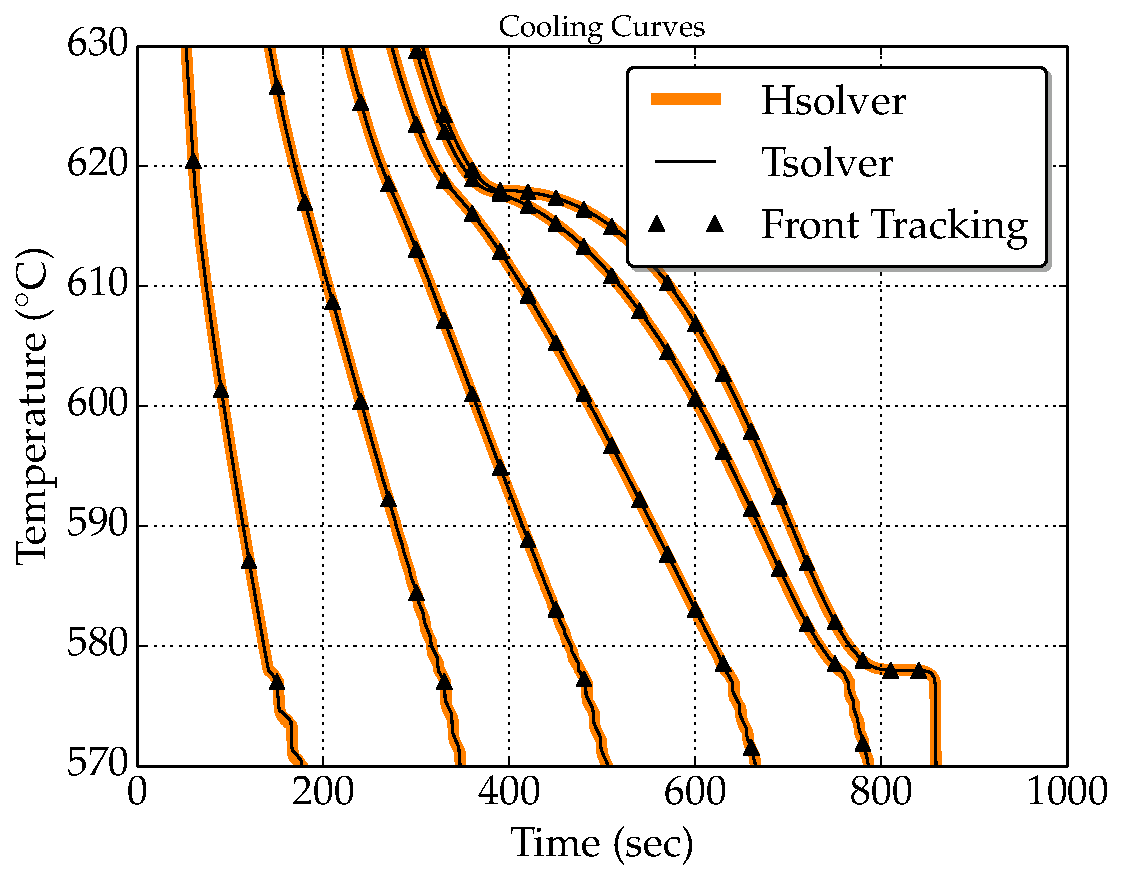
\includegraphics[width=\textwidth]{Chapter3/Graphics/diffusion/diffusion_CC.pdf}
	\caption{}
    \label{fig:validation_diffusion_CC}
  \end{subfigure}
  %------------------------------
  \vskip\baselineskip
  %------------------------------
  \begin{subfigure}[t]{0.7\textwidth}
    \centering
	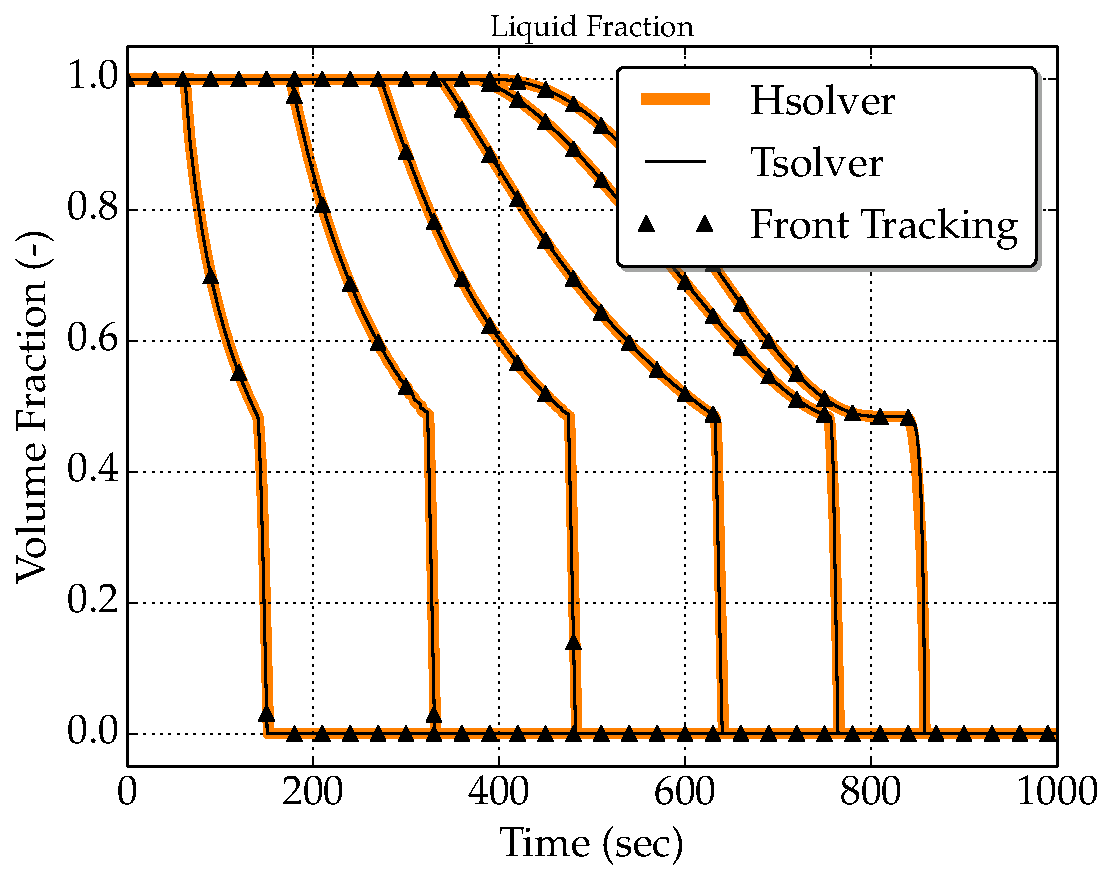
\includegraphics[width=\textwidth]{Chapter3/Graphics/diffusion/diffusion_LF.pdf}
	\caption{}
    \label{fig:validation_diffusion_LF}
  \end{subfigure}
   %------------
\caption{Computed unidirectional heat diffusion during solidification of an \bin{Al}{7}{Si} alloy 
using (orange) the enthalpy method and (black) the temperature method, comparison being made 
for (a) cooling curves  and (b) the liquid fraction history. 
Each curve corresponds to a position along the sample, from 0 cm (cooling 
side) to 10 cm (insulated side), with 2 cm spacing between the positions.
The reference solution by the Front Tracking method (values in shown by the triangular markers).} 
\label{fig:validation_diffusion}
\end{figure}
%------------------


%\subsection{Convection and diffusion}


\section{Application: multicomponent alloy solidification}
%==================
%
We have shown that the efficiency of the temperature-based resolution resides in its performance when combined with 
thermodynamic tabulations. A multicomponent alloy consists of at least two solute elements, and 
therefore the tabulation size increases, hence the number of search operations also increases. 
To demonstrate the speed-up ability of the temperature-based approach while predicting all phase 
transformations during macrosegregation caused solely by mass diffusion, we consider the solidification of a ternary alloy, \tern{Fe}{2}{C}{30}{Cr}.
In order to neglect fluid flow resolution, we assume that solidification in this case is so slow that no forces are generated inside the melt, while
additionally all buoyancy forces are also neglected, so no momentum conservation is solved in this section.

As illustrated in \cref{fig:mutlicomponent_geo}, the alloy domain has a cylinder shape close to 3-inch height $\times$ 1-inch diameter. 
Exact values are reported in \cref{table:ternary_data_case} with all material properties, initial and boundary conditions, 
as well as numerical parameters for the simulations. The melt steel is initially at \SI{1395}{\udegC}. The 
temperature of the bottom surface is imposed with a constant decreasing rate of \SI{0.1}{\uCR} starting 
with \SI{1380}{\udegC} as shown in \cref{fig:mutlicomponent_bc}, i.e. \SI{40}{\udegC} higher than the nominal liquidus temperature as shown 
in \cref{fig:ternary_nominalpath}. The other surfaces are kept adiabatic. 

The cylinder is held in a vertical position parallel to the gravity vector, the latter pointing downwards.
\cref{fig:ternary_nominalpath} also provides the transformation path of the alloy at nominal composition, i.e. assuming no macrosegregation and full 
thermodynamic equilibrium as computed with ThermoCalc and the TCFE6 database \citep{tcfe6_tcfe6:_2010, andersson_thermo-calc_2002}. 
A total of 5 phases need to be handled, the characteristic temperature for their formation being reported 
in \cref{fig:mutlicomponent_bc}.

%-----------------
\begin{figure}[htbp]
\centering
   %------------
  \begin{subfigure}[t]{1.0\textwidth}
    \centering
	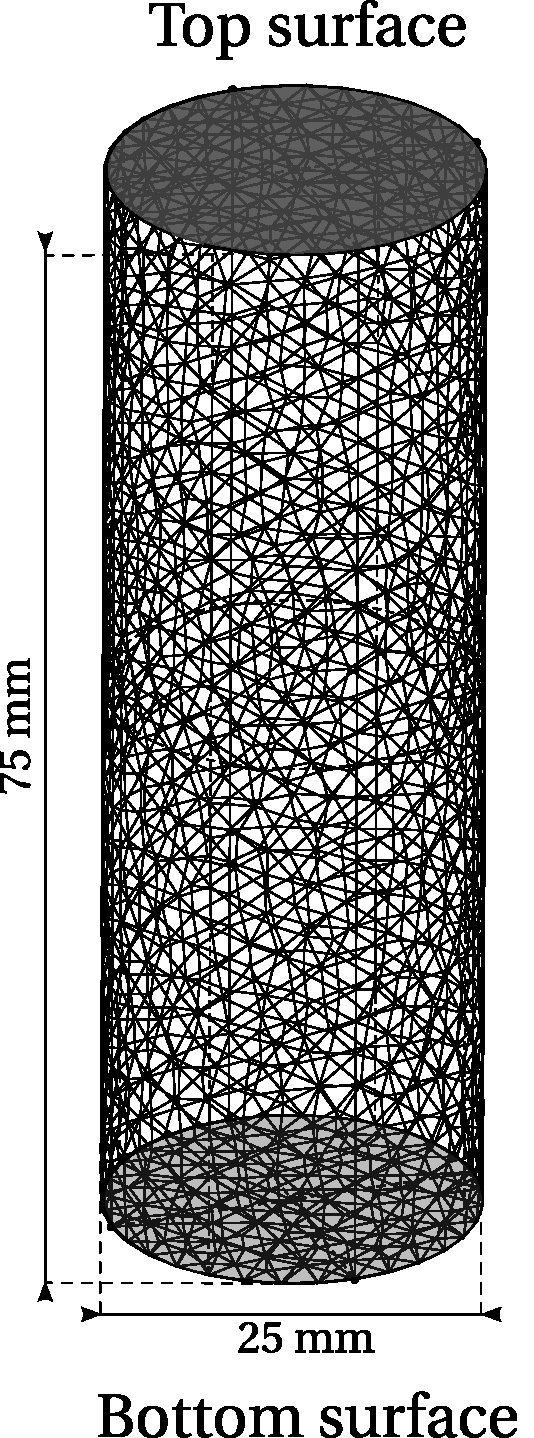
\includegraphics[width=0.25\textwidth]{Chapter3/Graphics/multicomponent/geo_bc/Cylinder_nocolor_annotate.pdf}
	\caption{}
    \label{fig:mutlicomponent_geo}
  \end{subfigure}
   %------------
    \vskip\baselineskip
   %------------
   \hspace{1mm}%\quad
   \begin{subfigure}[t]{1.0\textwidth}
    \centering
	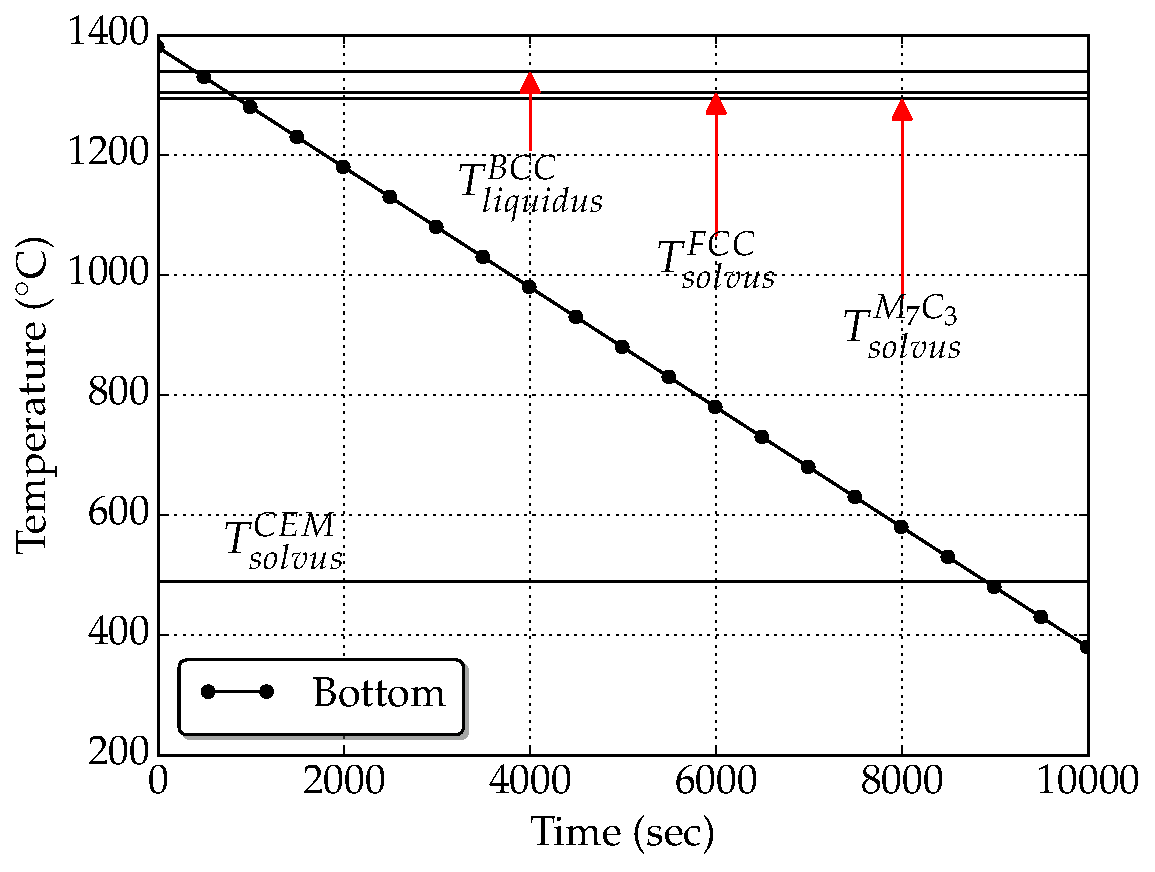
\includegraphics[width=0.75\textwidth]{Chapter3/Graphics/multicomponent/geo_bc/BC.pdf}
	\caption{}
    \label{fig:mutlicomponent_bc}
  \end{subfigure}
  %------------------------------
\caption{Configurations for upward directional casting of (a) a 1-inch diameter $\times$ 3-inches height cylindrical domain for which
(b) temperature-time conditions are imposed at its bottom surface.} 
\label{fig:mutlicomponent_geobc}
\end{figure}
%-----------------

%-------------------------
\subsection{Tabulations}
%-------------------------

Full thermodynamic equilibrium is considered in the present case. Due to macrosegregation, 
the average composition is expected to continuously vary in time and space during casting. 
Transformation paths are thus determined a priori for a set of average compositions around 
the nominal value. Hence, carbon content varies in the interval [\SI{1.8}{\ucomposition}, \SI{2.2}{\ucomposition}] 
while chromium content variation is in the interval [\SI{27}{\ucomposition}, \SI{33}{\ucomposition}]. The offset of $\pm$ 10\%  with 
respect to the nominal composition value allows tabulating relatively small composition steps
to ensure a fairly accurate mapping when compared to the corresponding ternary phase diagram. 

The average composition step is \SI{0.04}{\ucomposition} for carbon and \SI{0.6}{\ucomposition} for chromium, thus representing 2\% 
intervals with respect to the nominal composition. The temperature varies in the interval 
[\SI{100}{\udegC}, \SI{1600}{\udegC}] by \SI{5}{\udegC} steps. For each triplet (carbon content 
in \si{\ucomposition} C, ${w_\text{C}}_0$ , chromium content in \si{\ucomposition} Cr,  ${w_\text{Cr}}_0$, temperature in \si{\udegK}) 
corresponds a phase fraction $g^\phi$ and a pair of intrinsic phase composition ($\wC^\phi$,$\wCR^\phi$). For the 5 
phases listed in \cref{fig:ternary_nominalpath} (LIQ$\equiv$liquid, BCC$\equiv$ferrite, FCC$\equiv$austenite, 
$\carbide \equiv$carbide, CEM$\equiv$cementite), the enthalpy $\hphi$ and density $\rphi$, are tabulated 
as functions of temperature and phase intrinsic composition. If this latter input lies between two tabulated 
values, a linear interpolation is performed to determine the output, i.e. phase enthalpy and density. With 
the advancement of solidification, the liquid is enriched or depleted with solute by macrosegregation, which enables new 
solidification paths. It means that the primary solidifying phase is not necessarily the same as when considering 
the nominal composition. For this reason, the tabulation approach is interesting inasmuch as it provides phase 
transformation paths and values of phase properties that are compatible with the system’s actual composition. 

\Cref{fig:ternary_tabulations} summarises the tabulated thermodynamic data for two sets of average composition for the considered 
ternary system. Note that in the present test case, phase densities are taken constant ($\rhos=\rhol=$ \SI{6725}{\udensity}). 
Therefore they are not tabulated. With this assumption, no shrinkage occurs upon phase change.


%----------------------
\begin{figureth}
% textwidth 
{0.8}
%path 
{Chapter3/Graphics/multicomponent/SP_nominal.pdf}
% caption
{Thermodynamic mapping \citep{tcfe6_tcfe6:_2010, andersson_thermo-calc_2002} of the transformation 
path for the \tern{Fe}{2}{C}{30}{Cr} at nominal composition.}
% label
\label{fig:ternary_nominalpath}
\end{figureth}
%-----------------------------------


%=====================================BIG PORTRAIT FIGURE =====================================
\begin{figureth}
% textwidth 
{0.75}
%path 
{Chapter3/Graphics/multicomponent/tabulations/planche_tabulations_portrait.pdf}
% caption
{Tabulated thermodynamic data for the ternary system Fe-C-Cr alloy with software 
Thermo-Calc \citep{andersson_thermo-calc_2002}  with database TCFE6 \citep{tcfe6_tcfe6:_2010}.
The two columns represent two values of average composition, for a) low carbon and chromium content
and b) high carbon and chromium content.
The effect of their variation on transformation paths, phase compositions and phase enthalpies is shown in the corresponding graphs.}
% label
\label{fig:ternary_tabulations}
%\thispagestyle{headings}
\end{figureth}
%=====================================BIG PORTRAIT FIGURE =====================================



%----------------
\begin{tabulate}
%
% caption 
{Solidification parameters for the \tern{Fe}{2}{C}{30}{Cr} alloy.}
% label
{table:ternary_data_case}
% line separation (e.g. 1.5mm)
{0.6mm}
% column justification-number (e.g. |c|ll|)
{llll}
% header titles (should use the & sign to switch columns)
{\textbf{Parameter} & \textbf{Symbol} & \textbf{Value} & \textbf{Unit}}
% cells content (should use the & and // to switch columns and rows)
{
Nominal composition 			& ${w_\text{C}}_0$ 				& 2 					& \si{\ucomposition} 	\\ 
                    			& ${w_\text{Cr}}_0$ 			& 30 					& \si{\ucomposition} 	\\ 
Characteristic temperatures 	& $T_\text{bottom}$ 	& \cref{fig:mutlicomponent_bc}	 & \si{\udegC} \\ 
Phase fraction 					& $g^\phi$ 				& Tabulations \cref{fig:ternary_tabulations}	& $-$ 					\\ 
Phase enthalpy 					& $\h^\phi$ 			& Tabulations \cref{fig:ternary_tabulations}	& $-$ 					\\ 
Phase composition 				& $\wC^\phi$ 			& Tabulations \cref{fig:ternary_tabulations}	& \si{\ucomposition}  	\\ 
Phase composition               & $\wCR^\phi$ 			& Tabulations \cref{fig:ternary_tabulations}	& \si{\ucomposition}  	\\ 
Diffusion coefficients 			& $\avg{D_\text{C}}^l$ 	& \num{15e-10} 	& \si{\udiffusivity}  	\\ 
                        		& $\avg{D_\text{Cr}}^l$	 & \num{15e-10} 	& \si{\udiffusivity}  	\\ 
Dynamic viscosity  				& $\mul$ 					& \num{2e-3} 		& \si{\uviscosity}  	\\ 
Thermal expansion coefficient 	& \betaT 					& \num{8.96e-5} 	& \si{\ubetaT}  		\\ 
Solutal expansion coefficient 	& $\betawlC$ 				& \num{1.54e-3} 	& \si{\ubetawl}  		\\  
                              	& $\betawlCR$ 				& \num{1.72e-2} 	& \si{\ubetawl}  		\\ 
Thermal conductivity in the solid & $\ks$ 					& \num{40} 			& \si{\uconductivity}  	\\ 
Thermal conductivity in the liquid & $\kl$ 					& \num{28} 			& \si{\uconductivity}  	\\ 
Dendrite arm spacing 			& $\lambda$ 				& \num{60e-6} 		& \si{\metre}  			\\ 
Density 						& $\rholref$ 						& \num{6725} 	& \si{\udensity}  		\\ 
Reference composition (carbon)	&$\avg{w_\text{C}}_\text{ref}^l$	& \num{2} 		& \si{\ucomposition}  	\\
Reference composition (chromium)&$\avg{w_\text{Cr}}_\text{ref}^l$	& \num{30} 		& \si{\ucomposition}  	\\
Reference temperature 			&$\avg{w_\text{C}}_\text{ref}^l$	& \num{1377} 	& \si{\udegC}  	\\
\hline 
Initial temperature 	& $T_0$ & \num{1395}	& \si{\udegC}  \\ 
Ingot diameter 			&   	& \num{25e-3} 	& \si{\metre}  \\ 
Ingot length 			&   	& \num{75e-3} 	& \si{\metre}  \\ 
\hline 
FE mesh size 			&  		& \num{e-3} 	& \si{\metre}  \\ 
Time step 				& $\dt$ & \num{0.1} 	& \si{\second}  \\ 
Convergence criterion (residual) 	& $\varepsilon_R$ & \num{e-6} & $-$ \\ 
Convergence criterion (temperature) & $\varepsilon_T$ & \num{e-2} & \si{\udegK} 
}
%
\end{tabulate}
%-----------------


\subsection{Discussion}
%-----------------------
A first case is considered without macrosegregation, that is, all mechanical driving forces are bypassed, leading to a static melt. 
This is achieved by nullifying the thermal and solutal expansion coefficients, which is equivalent to a constant density in space 
and time, i.e. no Boussinesq force is considered. This way, the average composition may only vary due to diffusion in the liquid 
phase.
%according to \cref{eq:diag_solute} where the convection term is neglected. 

Diffusion is significantly small in the present case and can be 
neglected too. The composition distribution thus maintains a homogeneous aspect throughout the sample during the entire 
cooling sequence. The phase transformations then are necessarily expected to follow the unique path shown in \cref{fig:ternary_nominalpath}. After 407 s 
of cooling, the liquidus isotherm enters the bottom surface of the geometry and starts its upward propagation, marking the solidification 
onset. 

\Cref{fig:planche_nomacroseg} presents the simulation results at 3 successive times for the distribution of the solute species and the temperature, as 
well as for the fraction of phases listed in \cref{fig:ternary_nominalpath}. At 600 s, a fully liquid region is still largely present while the mushy zone is 
made of liquid plus the primary solid phase (ferrite). At \num{10560} s, the sample is fully solid, with fractions of ferrite and cementite that 
corresponds to the values read in \cref{fig:ternary_nominalpath} at low temperature. At the selected intermediate time, the presence of 4 phases is found. The 
solid region at the bottom of the cylinder is made of ferrite, austenite plus carbide, the temperature being still too high to permit the 
cementite to form. The mushy zone above the solid region is characterized by the presence of 3 phases due to a peritectic reaction taking 
place that progressively transform ferrite into austenite in the presence of liquid. 

It can be noticed that the phase fraction isovalues 
in \cref{fig:planche_nomacroseg} (at 600 s) are horizontal, owing this to two factors: the first is the temperature field, which varies unidirectionally from 
bottom to top, controlled by thermal diffusion, while the second is the uniform average composition throughout the sample due to the absence 
of convection. In fact both factors are consequences of the flow absence, which would transport heat and solute by advection, thus inevitably 
changing the phase distribution. The succeeding phase change is a solid-state transformation where $\alpha$-ferrite and the carbide $\carbide$ react to form 
cementite after cooling below \SI{490}{\udegC}, as shown in \cref{fig:mutlicomponent_bc}. The reaction is relatively slow, ending with 28\% 
of cementite and 72\% of $\alpha$-ferrite.

%=====================================BIG LANDSCAPE FIGURE =====================================
\begin{landscape}
\begin{figureth}
{1.2}
{Chapter3/Graphics/multicomponent/planche_nomacroseg.pdf}
{Upward solidification of a cylinder rod with a static liquid at 
3 stages in a \tern{Fe}{2}{C}{30}{Cr}. The left columns show the average 
composition and temperature distribution, while the right columns show the phase fractions.}
\label{fig:planche_nomacroseg}
%\thispagestyle{headings}
\end{figureth}
\end{landscape}
%=====================================BIG LANDSCAPE FIGURE =====================================

\clearpage
\section*{Résumé chapitre 3}

Ce chapitre reprend les détails du solveur pour la conservation d'énergie avec changement de phase utilisé au CEMEF.
Celui-ci est basé sur une méthode enthalpique, dénommée \emph{Hsolver}, dont la variable principale est l'enthalpie
moyenne volumique du système, $\avg{\rho h}$. Ce solveur est aussi compatible avec des données tabulées provenant de bases de données
thermodynamiques, fournissant des valeurs précises pour chaque phase $\phi$ présente au moment de la transformation: 
fraction $\gphi$, composition intrinsèque $\wiphi$, enthalpie massique $\hphi$ et densité $\rphi$. 
Avec ces données, l'équation de conservation de l'énergie est résolue dans son état nonlinéaire 
provenant de la dépendance de $\rho h$ par rapport aux propriétés citées précédemment, sachant que celles-ci varient
aussi en fonction de la composition moyenne du volume élémentaire représentatif.


Cependant, la résolution \emph{Hsolver} nécessite une lourde recherche itérative à chaque pas de temps, consistant à convertir
$\avg{\rho h}$ en température $T$ pour évaluer le résidu du système nonlinéaire. Cette conversion est dénommée \emph{H2T} et elle est
compliquée du fait que les bases thermodynamiques fournissent la température comme donnée d'entrée, ce qui nous oblige de faire 
la recherche inverse itérative.


Dans ce chapitre, on propose de remplacer la conversion \emph{H2T} par une autre, \emph{T2H}. Comme son nom l'indique,
on part de l'idée que la température soit la variable principale du système et on devrait alors trouver l'enthalpie moyenne volumique
à chaque pas de temps. Avec ce changement, on propose donc une nouvelle formulation éléments finis, \emph{Tsolver}, mettant en évidence les principales
différences algorithmiques des deux résolutions.


Nous validons la formulation \emph{Tsolver} dans un cas purement diffusif et comparé à des calculs faits avec la méthode \emph{Hsolver}, 
ainsi qu'une comparaison avec une solution numérique obtenue par une méthode de suivi de front \citep{gandin_constrained_2000}.
Enfin, nous montrons une application de solidification dirigée d'un système ternaire, \tern{Fe}{0.2}{C}{30}{Cr}, en régime diffusif.

% avec une analyse de la ségrégation en peau et en coeur de la pièce. % resume francais
